% !Mode:: "TeX:UTF-8"%確保文檔utf-8編碼
\documentclass[border=2pt]{standalone}
\usepackage{tikz}
\usepackage{pgfplots}
\usetikzlibrary{intersections,calc,positioning}
\usetikzlibrary{shapes.geometric}%菱形
\pgfplotsset{compat=newest}


\begin{document}
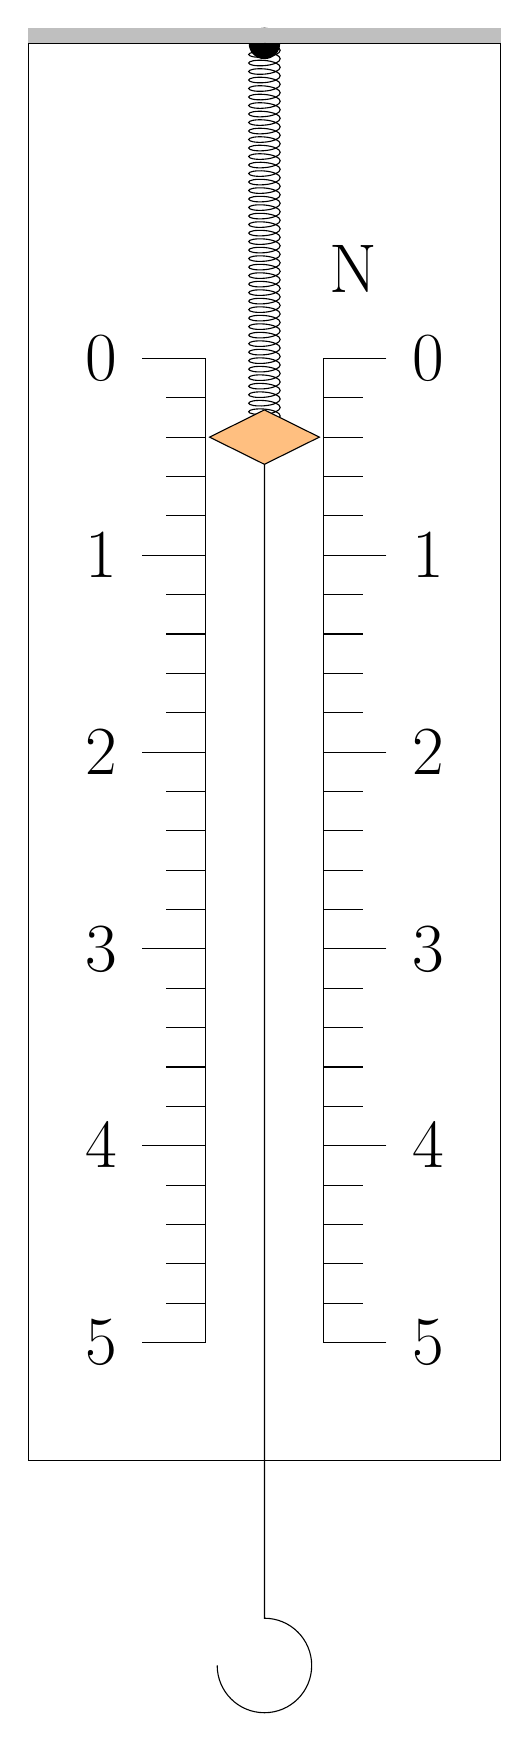
\begin{tikzpicture}
%力的数值
\def\forcenum{0.4}
\def\forcepoint{-10*\forcenum/4}
\pgfmathsetmacro{\coilsegmentlen}{1+\forcenum/5}
%刻度
\begin{scope}[scale=0.5]
%主线轴
\def\starty{0}
\def\endy{-25}
\pgfmathsetmacro{\stepy}{\starty-1}
\pgfmathsetmacro{\stepyfive}{\starty-5}
\pgfmathsetmacro{\stepyten}{\starty-10}

\coordinate (startpoint) at (1.5,\starty) ;
\coordinate (endpoint) at (1.5,\endy) ;
\draw [](startpoint) -- (endpoint);


%细小刻度
\foreach \x in {\starty,\stepy,...,\endy}
  \draw [](1.5,\x) -- (2.5,\x) ;   

%5分之一刻度
%\foreach \y in {\starty,\stepyfive,...,\endy}
%  \draw [] (1.6,\y) -- (0,\y);


%10分之一刻度
\foreach \i in {\starty,\stepyfive,...,\endy}
  \draw [] (3.1,\i) -- (1.5,\i)%2.2
  node[right=1cm] {\Huge \pgfmathprint{int(-\i/5)}};
\end{scope}




%翻转
\begin{scope}[scale=0.5,xscale=-1]

%主线轴
\def\starty{0}
\def\endy{-25}
\pgfmathsetmacro{\stepy}{\starty-1}
\pgfmathsetmacro{\stepyfive}{\starty-5}
\pgfmathsetmacro{\stepyten}{\starty-10}

\coordinate (startpoint) at (1.5,\starty) ;
\coordinate (endpoint) at (1.5,\endy) ;
\draw [](startpoint) -- (endpoint);


%细小刻度
\foreach \x in {\starty,\stepy,...,\endy}
  \draw [](1.5,\x) -- (2.5,\x) ;   

%5分之一刻度
%\foreach \y in {\starty,\stepyfive,...,\endy}
%  \draw [] (1.6,\y) -- (0,\y);


%10分之一刻度
\foreach \i in {\starty,\stepyfive,...,\endy}
  \draw [] (3.1,\i) -- (1.5,\i)%2.2
  node[left=1cm] {\Huge \pgfmathprint{int(-\i/5)}};
\end{scope}



%额外的修改
%外边框
\draw (-3,-14) rectangle (3,4);
\fill (0,4) circle (0.2);
\fill[gray!50] (-3,4) rectangle (3,4.2);
%unit
\node [above right=1cm] {\Huge N};
%上面的弹簧
\draw[decoration={aspect=0.3, segment length=\coilsegmentlen mm, amplitude=2mm,coil},decorate] (0,4) -- (0,\forcepoint); 

%菱形指针和下面的钩子
\draw (0,\forcepoint) -- +(0,-15)  arc (90:-180:0.6);
\node [draw,scale=2,diamond,fill=orange!50,aspect=2] at (0,\forcepoint) {}; 




\end{tikzpicture}
\end{document}